\section{Preliminaries}
\label{sec:preliminaries}

The vocabulary used throughout this document is described in the Glossary \cite{glossary} (e.g., \emph{subnets}, \emph{actors}, \emph{accounts}, \emph{users}, and \emph{\ipc agents}).
The reader is assumed to be familiar with the terminology defined there.
\jorge{Despite this note, the vocabulary seems to be defined throughout the body. If we're defining in the body anyway, the appendix seems redundant -- this isn't a book.}
\marko{If the glossary is stable, I suggest bringing it to the main body of the paper by defining concepts inline, as we go. Glossary can additionally stay in the appendix, for quick reference.}

% \subsection{Computation and failure model}

% We model \ipc as a distributed (``message-passing") system consisting of \emph{processes} that communicate by exchanging \emph{messages}%
% \footnote{Network messages are not to be confused with Filecoin actor messages, to which this document refers as transactions.}
% over a network. 
% In practice, a process is a program running on a computer, having some state, and reacting to external events and messages received over a communication network.
% We describe processes as exemplified in \Cref{alg:process-definition}.

% \begin{algorithm}[H]
% \footnotesize
% \caption{Process definition.}\label{alg:process-definition}
%   \DontPrintSemicolon
%   \SetKwProg{Component}{$\blacktriangleright$ \bf}{:}{\KwRet}
%   \SetKwFor{UponKW}{upon}{do}{fintq}
%   \SetKw{Trigger}{trigger}
%   variableA = initial value\\
%   variableB = initial value\\ \jorge{this is kind of a weird notation, as you can't tell whether you're defining a new variable or just assigning a new value}
%   ...\\
%   \Component{process}{
%      \UponKW{event(params...)}{
%        \tcp{Logic to execute atomically}
%      }
%      \UponKW{event(params...)}{
%        \tcp{Logic to execute atomically}
%      }
%      ...
% }
% \end{algorithm}

% A process that performs all the steps exactly as prescribed by the protocols in which it is participating is \emph{correct}.
% A process that stops performing any steps (i.e., \emph{crashes}) or that deviates from the prescribed protocols in any way is \emph{faulty}.
% If a process is correct or may only fail by crashing, it is \emph{benign}.
% A non-benign process is \emph{malicious}.
% \matej{We can remove terms we end up not using...}

% In general, faulty processes can be malicious (Byzantine): we do not put any restrictions on their behavior, except being computationally bounded and, thus, unable to subvert standard cryptographic primitives, such as forging signatures or inverting secure hash functions.
% If the implementation of some component in our design requires additional assumptions on the behavior of faulty processes, they will be stated explicitly.
% % We do not make a general statement about the fault tolerance of \ipc as a system, as to how many faulty processes the system can sustain.
% % This depends on the final implementation of its components.

% We use the term \emph{participant} to describe an entity participating in the system that controls one or more processes.
% All processes controlled by one participant are assumed to be in the same trust domain, that is, they assume one another's correctness.
% For example, a participant in the child subnet will probably run multiple processes:
% one for participating in the child subnet (child replica),
% one for participating in the parent subnet (parent replica),
% and one that processes the information from the two replicas and submits transactions accordingly (\ipc agent).
% We precisely define the replicas and the \ipc agent (all of them being processes) in \Cref{sec:components,sec:smr}.
% The \ipc agent of a participant always assumes that the information it receives from "its own" child replica is correct.
% However, messages received from another participant's replica or \ipc agent are seen as potentially malicious.

% The synchrony assumptions may vary between different components of \ipc.
% We thus state those assumptions whenever necessary, when describing concrete implementations of \ipc components.

% \subsection{State machine replication (SMR) and \actors}
% \label{sec:smr}

% \paragraph{SMR and replicated state.}
% A \emph{state machine replication (SMR) system}%
% is a system consisting of processes called \emph{replicas}, each of which locally stores a copy of (or at least has access to) \emph{replicated state}
% that it updates over time by applying a sequence of \emph{transactions} to it. 
% \jorge{it's not objectively wrong, but not a huge fan of defining replicas now, after they were mentioned several times}
% Without specifying the details, we assume that any process can \emph{submit} a transaction to an SMR system (we call such a process an \emph{SMR client})
% and that this transaction will eventually be ordered and applied to the replicated state.
% We call an SMR system that is part of \ipc a \emph{subnet}.

% An SMR system guarantees to each correct replica that, after applying $n$ transactions to its local copy of the replicated state,
% the latter will be identical to any other correct replicas' copy of the replicated state after applying $n$ transactions.
% The replicas achieve this by executing an \emph{ordering protocol} to agree on a common sequence of transactions to apply to the replicated state.

% Note that replicas do not necessarily all hold the same replicated state at any instant of real time,
% since each replica might be processing transactions at a different time.
% In this context, there is no such thing as “the current replicated state of the SMR system”.
% There is only the current replicated state of a single replica.
% The replicated state of the system is only an abstract, logical construct
% useful for reasoning about transitions from one replicated state to another,
% happening at individual replicas by applying transactions (at different real times).
% When referring to a “current” replicated state, we mean the state resulting from the application of a certain number of transactions to the initial state.

% \paragraph{Actors.}
% The replicated state of an SMR system can be logically subdivided into multiple \emph{\actors}.
% A \actor is a portion of the replicated state with well-defined semantics.
% It defines the logic that a replica needs to execute when applying transactions and the new state that results from it.

% We model a \actor as a logical object in the replicated state that contains arbitrary variables representing its state.
% Its associated logic reacts to \emph{events} triggered by (1) the application of transactions or (2) the execution of other (or even own) actor logic. \jorge{why "even own"? why is that more surprising than foreign actor logic?}
% We describe actors as exemplified in \Cref{alg:actor-definition}. \jorge{Is it a definition or an example?}


% \begin{algorithm}[H]
% \footnotesize
% \caption{\actor definition}\label{alg:actor-definition}
%   \DontPrintSemicolon
%   \SetKwProg{Component}{$\blacktriangleright$ \bf}{:}{\KwRet}
%   \SetKwFor{UponKW}{}{}{fintq}
%   \SetKw{Trigger}{trigger}
%   variable = initial value\\
%   variable = initial value\\
%   ...\\
%   \Component{\actor name}{
%      \UponKW{Function(params...)}{
%        \tcp{Logic to execute}
%      }
%      \UponKW{Function(params...)}{
%        \tcp{Logic to execute}
%      }
%   }
% \end{algorithm}
% While \emph{process} denotes an instance of a program running on some physical machine,
% \actors are an abstraction over the replicated state of an SMR system and their logic is being executed by all its replicas.
% While a process can submit a transaction to an SMR system, a \actor cannot.

\paragraph{Basic abstractions.}
A \emph{subnet} consists of multiple \emph{replicas}, yet we abstract a subnet as a single entity which maintains an  abstraction of \emph{replicated state} (of which each replica maintains a copy)
that can only be modified through transactions submitted either by \emph{users} or by an \emph{\ipc agent}.
It is the state (and only the state) that all replicas agree on.
\akosh{What about cron, and similar end-of-epoch changes? Although I saw cron will be removed from Filecoin.}
\jorge{There are proposals to fix some cron issues (https://github.com/filecoin-project/FIPs/discussions/638),
but I don't think the current direction is towards removing it; in fact, I think there are very strong opinions against that solution.}
\matej{Even that must be bound to blocks. As I understand it, it is some actions triggered every k blocks.
That can be easily modeled by every k-th block containing an (implicit) transaction triggering the action (submitted by some implicit system-level user).}
We further abstract away the concrete mechanism of transaction submission and execution, as it is specific to the implementation of each particular subnet.

For example, the replicated state of a subnet representing a game of chess would consist of the player identities, a flag indicating which player's turn it is, and positions of the individual pieces on the board,
while players' moves would be performed by submitting transactions to the subnet.

\paragraph{Interaction between subnets.}
In \ipc, the replicated state (or, simply, state) of one subnet often needs to react to changes in the state of another subnet.
E.g., after a game hosted in a subnet finishes, the implementation of the game logic might need to update the involved players' rankings in its parent subnet based on the result of the game.
As the state of every subnet evolves independently of the state of other subnets,
\emph{IPC establishes a protocol for interaction between the states of different subnets}.

At the basis of the protocol, IPC relies on  \emph{\pofsFull ({\pof}s)}.
In a nutshell, a \pof is data that proves that a subnet irreversibly reached a certain replicated state.
Regardless of the approach to \emph{finality} that the  \emph{ordering protocol} of a subnet uses (e.g., immediate finality for classic BFT protocols \cite{}, or probabilistic finality in PoW-based systems \cite{Bitcoin}),
a \pof serves to convince the verifier that the replicated state the \pof refers to will not be rolled back. This helps IPC establish the partial ordering between the states of two subnets. 


For example, for a subnet using a BFT-style ordering protocol, a quorum of signatures produced by its replicas can constitute a \pof.
\marko{what about longest chain style protocols, how do we construct \pof there?}
To prove the finality of the state of a subnet based on a longest-chain-style protocol,
a \pof might consist of signatures of a committee of processes considering the state deep enough (for some parametrized notion of ``deep enough'') in the chain.
This committee can be, for example, a quorum of replicas of the very subnet that is to verify the \pof.
If the verifying subnet itself is a longest-chain one, a \pof can be as simple as a hash of the proving subnet's block,
with every replica of the verifying subnet deciding locally about the \pof's validity (potentially leading to forks in the worst case).

If a \pof is associated with subnet \subnetName{A}'s replicated state at \emph{block height} $h_\subnetName{A}$,
and the \pof is included in subnet \subnetName{B}'s replicated state at block height $h_\subnetName{B}$,
then subnet \subnetName{B}'s replicated logic will consider all \subnetName{A}'s state changes up to $h_\subnetName{A}$
to have occurred at \subnetName{B}'s height $h_\subnetName{B}$.
(Unless, of course, another \pof' of $h'_\subnetName{A}$ has been included by \subnetName{B} at $h'_\subnetName{B}$,
in which case \subnetName{B} consideres only the state changes between $h'_\subnetName{A}$ and $h_\subnetName{A}$ to have occured at $h_\subnetName{B}$).

In the following, for some representation of a subnet's replicated state (e.g., its full serialization or a handle that can be used to retrieve it in a content-addressable way, such as an IPFS content identifier (CID)),
we denote by {\pof}($state$) the proof that a subnet reached $state$.

\marko{but what if it is - esp at longest chain parent net?}
\arp{what happens if state is rolled back before a checkpoint for example?. If we are talking about payments, if checkpoint occurred and then state rolled back then whoever got its money back (due to the rollback) cannot withdraw that money to the parent anymore. If we are talking about state then behavior is undefined.}
\matej{If the state is rolled back despite a \pof, then the assumptions underlying the verification of the \pof were wrong and the verifier treats the subnet as faulty (e.g. the same way as if the adversary started controlling the majority of its replicas / conputing poser / stake ...)}
\akosh{There's always that word "assume"... perhaps what's missing from the defintion of PoF is that violations are detectable, e.g. by checkpointing.}
\matej{Are they though in all the imaginable cases? I'm not quite sure. I assume that by ``violation'' you mean a state with a valid \pof being rolled back. Is that the case?}
\jorge{I think I +1 Akosh on "assume". If we're saying a rollback is a violation, then this isn't a question of assumptions -- it's a question of definition. Something like "... proof that a subnet reached $state$ and cannot be rolled back without triggering a violation."?}.
\matej{I just removed the second part of the sentence to avoid this confusion. It's quite clear from the definition of a \pof (it "convinces the verifier that the state will not be rolled back") and removes the necessity of any kind of assumptions. I.e., only the verifier locally makes whatever assumptions they need to be reasonably "convinced" by the \pof.}
We also denote by {\pof}(\tx{tx}) the proof that a subnet reached a state in which transaction \tx{tx} already has been applied to the replicated state.

\paragraph{Naming subnets.}
We assign each subnet a name that is unique among all the children of the same parent.
Similarly to the notation used in a file system, the name of a child subnet is always prefixed by the name of its parent.
For example, subnets \subnetName{P/C} and \subnetName{P/D} would both be children of subnet \subnetName{P}.

\paragraph{Notation.} We refer to an account \accountName{a} in the replicated state of subnet \subnetName{S} as \subnetName{S}.\accountName{a}.
To denote a function of an actor in the replicated state of a subnet, we write \funcNameFull{Subnet}{Actor}{Function}.
E.g., the \emph{IPC Gateway Actor} (\gw) function \funcName{CreateChild} in subnet \subnetName{P} is denoted \funcNameFull{P}{\gw}{CreateChild}.
We also use this notation for a transaction \tx{tx} submitted to subnet \subnetName{P} that invokes the function, e.g., \tx{tx} = \funcNameFull{P}{\gw}{CreateChild}$(\subnetName{P/C}, params)$.

\paragraph{Representing value.}
For each pair of subnets in a parent-child relationship, we assume that there exists a notion of \emph{value} (measured in \emph{coins}) common to both subnets.%
\footnote{One can easily generalize the design to decouple the use of value between a parent and its child, but we stick with using the same kind of value in both subnets for simplicity.}
We represent this value by associating some number of coins (also referred to as funds) with accounts and actors in a subnet's replicated state.
Each user is assumed to have an account in each subnet the user interacts with.
All the transactions spending coins from an account must be signed by the corresponding user's private key.
For simplicity of presentation, we do not explicitly include these signatures in the further description of \ipc.

We also assume that the submission, ordering, and application of transactions is associated with a cost (known as transaction fees, or \emph{gas}).
Each subnet client (user wallet or IPC agent) submitting a transaction to a subnet must have an account in that subnet, from which this cost is deducted.
If the funds are insufficient, the subnet may fail to execute the transaction.

Note that the operation of \ipc requires the submission and processing of transactions that are not easily attributed to a concrete user.
This is the case with transactions that an \ipc agent submits on behalf of a whole subnet.
We discuss incentivization of participants to run \ipc agents and pay for the associated transaction fees in \Cref{sec:refunds-rewards}.
\TODO{Move this part after \ipc agent and actors, as it already uses thos terms.}

\paragraph{\ipc actors.}
For inter-subnet communication, \ipc relies on two special types of actors: the \gwFull (\gw) and the \saFull (\sa).
In a nutshell, their functions are as follows.
\begin{enumerate}
    \item The \gw is an actor that contains all \ipc-related information and logic associated with a subnet that needs to be replicated \emph{in the subnet itself}.
    Each subnet contains exactly one \gw. We describe the \gw in detail in \Cref{sec:gw}
    \marko{Why is IGA an actor an not a blob of information? When does the state of IGA need to change (to demonstrate the need of IGA to be an actor) and how does it change (governance)?}
    \matej{Those questions should be answered in \Cref{sec:gw}}

    \item The \sa is the \gw's parent-side counterpart, i.e., it is an actor in a parent subnet's replicated state,
    containing all the data and logic associated with a particular child subnet -- we say the \sa ``governs'' that child subnet.
    A subnet contains as many \saFulls as the number of its children.
    We refer to the \sa governing child subnet \subnetName{C} as \saOf{C}.
    We describe the \sa in detail in \Cref{sec:sa}.

\end{enumerate}

\paragraph{\ipc agent.}

The \ipc agent is a process that mediates the communication between a parent and a child.
It has access to the replicated states of both subnets and acts as a client of both subnets.
When the replicated state of subnet \subnetName{A} indicates the need to communicate with subnet \subnetName{B},
the \ipc agent constructs a \pof for \subnetName{A}'s replicated state and submits it as a transaction to \subnetName{B}.

\ipc does not prescribe who must run an \ipc agent, nor how the \pof is to be constructed, nor which \ipc agent must submit the transaction with the \pof.
All this is specific to the implementation of the subnets involved.
The \ipc agents may run a protocol for choosing which of them submit(s) the transaction or even resort to a simplistic approach where each \ipc agent submits an identical transaction.
In our current implementation, for example, we construct the \pof directly in the verifying subnet's (\subnetName{B}'s) replicated state,
using one \ipc agent per replica of the proving subnet (\subnetName{A}).
When describing the functionality of \ipc and referring to ``the \ipc agent'' submitting a \pof,
we assume such a subnet-specific mechanism for choosing one (or multiple) \ipc agent(s) to perform the actual submission.

The interaction between subnets through \ipc agents is depicted in \cref{fig:interfaces}.

\begin{figure}[ht]
     \centering
     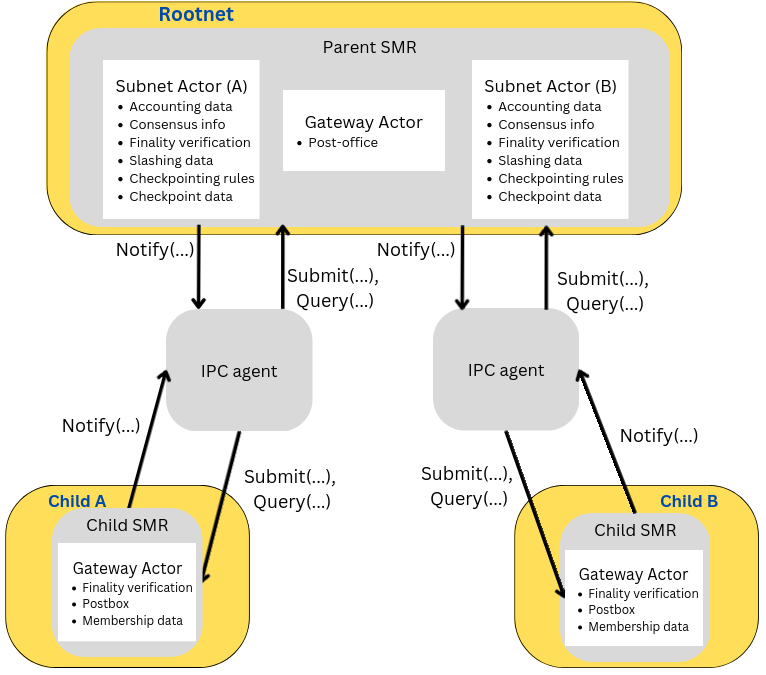
\includegraphics[width=0.75\textwidth]{compsintf-2subnets}
     \caption{The basic \ipc components and their interfaces in an example with one parent and 2 child subnets (A and B). \TODO{Update figure to be consistent with new notation.}}
     \label{fig:interfaces}
 \end{figure}

\paragraph{Incentives}

In general, submitting transactions (and their subsequent execution by the subnet) is associated with a \emph{cost} (often referred to as "gas").
We refer to the cost associated with a transaction as the \emph{transaction fee}, measured in coins.
A participant running an IPC agent is not necessarily interested in participating in such a costly protocol without incentives.
Moreover, the replicas of a subnet might need to cooperate with IPC agents during the construction of \pofsFull.
Even though certain deviations from the protocol can be detected and penalized (see \Cref{sec:slash}),
participants running subnet replicas might also need positive incentives to participate in the creation of a \pof.

The key to providing incentives for \ipc agents and replicas is that the \sa and the \gw can,
as actors, also hold funds that their logic can distribute among other accounts or actors on their respective subnets.
Thus, when an \ipc agent submits a transaction to one of these actors, they can be configured to reimburse (potentially adding an extra reward)
the account from which the transaction fee was paid (i.e., an account associated with the \ipc agent)%

The source of funding for the \gw and / or \sa is subnet-specific.
For example, a subnet’s implementation can require a certain part of each transaction fee to be sent to the subnet's \gw.
An \sa can be funded, for example, through transfers (withdrawals) of funds from the child subnet, or by charging a fees for propagating cross-net transactions.

To incentivize the replicas of a subnet to collaborate with the IPC agent on the creation of \pofsFull, a similar mechanism can be deployed.
For example, a valid \pof would include metadata, where the replicas that participated in its creation could insert an address to receive a reward when the \pof is accepted.

\TODO{Add example of gaming system incentives: The replicas and \ipc agents running the \subnetName{L2} subnet might get a commission from transaction fees,
while the single-game subnets might not need explicit incentivization at all, as they are mostly run by players, whose incentive is being able to play the game.}

\TODO{Matej: Describe firewall property (and trust model in general).}

\marko{What is missing here is a trust model - sth like an expanded slide 12 in} \url{https://docs.google.com/presentation/d/1l-wEprVrUQFvOjn_eV_QeAZqy6xy1Z7nnKS42zRMH-w/edit#slide=id.g10e8b8656ea_0_65}. It needs to be clear why do we need BFT in the first place and who trusts whom.